\documentclass[11pt]{amsart}
\usepackage[letterpaper, margin=1in]{geometry}
\usepackage{algorithm, algpseudocode}
\usepackage{float}
\usepackage{caption}
\usepackage{amsmath, amssymb, amsthm, amsaddr}
\usepackage{enumerate, subcaption, graphicx, hyperref}
\usepackage{color}
\title{AMATH 482: Homework 5 --- FCN vs. CNN under Weight Budget Constraints}
\author{Rohan Pandey}
\address{University of Washington, Seattle, WA \\ \texttt{rpande@uw.edu}}
\date{\today}

\begin{document}

\begin{abstract}
In this project, we investigate image classification on the Fashion-MNIST dataset using deep neural networks under strict parameter budget constraints. We implement and compare Fully Connected Networks (FCNs) and Convolutional Neural Networks (CNNs) with approximately 50K, 100K, and 200K parameters for FCNs, as well as CNN variants with budgets of roughly 10K, 20K, 50K, and 100K parameters. Our study includes extensive hyperparameter tuning, data augmentation, and regularization techniques to optimize performance while balancing accuracy and computational efficiency. In addition, we visualize training dynamics, intermediate feature maps, and synthesized class images to gain further insights into network behavior.
\end{abstract}

\maketitle

\section{Introduction and Overview}\label{sec:introduction}
Image classification is a cornerstone task in computer vision, with recent advances driven by deep learning techniques. In this project, we explore two popular architectures for classifying images from the Fashion-MNIST dataset: Fully Connected Networks (FCNs) and Convolutional Neural Networks (CNNs). Unlike conventional methods, our approach enforces strict weight budget constraints---approximately 50K, 100K, and 200K parameters for FCNs, and similarly constrained CNN variants. This not only forces the models to learn compact representations but also provides insight into the trade-offs between model complexity, accuracy, and training efficiency. In addition to standard training and evaluation, we include visualization techniques to examine feature maps and generate synthesized images representative of each class using gradient-based optimization.

\section{Theoretical Background}\label{sec:theory}
Deep neural networks are designed to learn hierarchical representations of data through a series of linear transformations and non-linear activations. Two common architectures for image classification are Fully Connected Networks (FCNs) and Convolutional Neural Networks (CNNs).

\subsection*{Fully Connected Networks (FCNs)}
FCNs consist of layers in which every neuron is connected to every neuron in the subsequent layer. While this design is straightforward, it can lead to a large number of parameters. Under a strict weight budget, the number of hidden units must be carefully selected. In an FCN, an input image is first flattened into a vector (e.g., a 28x28 image becomes a 784-dimensional vector). Each layer computes a linear transformation:
\[
\mathbf{z} = \mathbf{W}\mathbf{x} + \mathbf{b},
\]
followed by a non-linear activation function such as the Rectified Linear Unit (ReLU):
\[
\text{ReLU}(x) = \max(0, x).
\]
For classification tasks, the final layer outputs logits that are then transformed into a probability distribution using the softmax function:
\[
\sigma(\mathbf{z})_i = \frac{e^{z_i}}{\sum_{j=1}^{C} e^{z_j}},
\]
where \( C \) is the number of classes. The network is trained by minimizing the Cross-Entropy Loss:
\[
\mathcal{L} = -\sum_{i=1}^{C} y_i \log\big(\sigma(\mathbf{z})_i\big),
\]
which quantifies the dissimilarity between the predicted probability distribution and the true labels \cite{Goodfellow-et-al-2016}.

\subsection*{Convolutional Neural Networks (CNNs)}
CNNs are specifically designed to process spatial data like images. Convolutional layers apply learnable filters to local regions of the input, capturing spatial patterns while drastically reducing the number of parameters compared to FCNs. The convolution operation is defined as:
\[
(\mathbf{I} * \mathbf{K})(i,j) = \sum_{m} \sum_{n} \mathbf{I}(i-m, j-n)\mathbf{K}(m, n),
\]
where \(\mathbf{I}\) is the input image and \(\mathbf{K}\) is the convolution kernel. In addition to the kernel size, two important parameters in convolutional layers are the \textbf{stride} and \textbf{padding}. 

\textbf{Stride} refers to the step size with which the convolutional kernel moves across the input image. A stride of 1 means the filter is applied at every possible location, while a larger stride results in a down sampled output feature map. 

\textbf{Padding} involves adding extra border pixels (commonly zeros) around the input image. This can help control the spatial dimensions of the output feature maps. For instance, \emph{same} padding is used to preserve the input dimensions, whereas \emph{valid} padding (no padding) typically reduces the output size. These mechanisms are essential for designing deep architectures with controlled feature map sizes \cite{Goodfellow-et-al-2016}.

Pooling layers (e.g., max pooling) further reduce the spatial dimensions, leading to a compact representation that is subsequently fed into fully connected layers. CNNs typically employ techniques such as batch normalization and dropout to improve training stability and prevent overfitting \cite{srivastava2014dropout}.

\subsection*{Regularization and Weight Initialization}
Regularization techniques are essential to mitigate overfitting, particularly in high-capacity models. \textbf{Dropout} randomly deactivates a fraction of neurons during training, promoting redundancy and reducing reliance on specific neurons. In addition, robust weight initialization is crucial for effective training. Methods such as Xavier (Glorot) initialization and Kaiming (He) initialization maintain consistent variances of activations across layers, preventing issues like vanishing or exploding gradients \cite{he2015delving}. These strategies, combined with parameter budget constraints, encourage the network to develop efficient and compact representations while still achieving high performance.

\section{Algorithm Implementation and Development}\label{sec:algorithms}
Below is a high-level algorithm outlining the main steps of our project.

\begin{algorithm}[H]
    \caption{Training and Evaluation of FCN and CNN Models under Weight Budgets}
    \begin{algorithmic}[1]
        \State \textbf{Input:} Fashion-MNIST dataset, parameter budgets, hyperparameters (\texttt{learning\_rate}, \texttt{epochs}, \texttt{batch\_size})
        \State \textbf{Output:} Trained models and performance metrics
        
        \State \textbf{/* Data Loading and Preprocessing */}
        \State Download and normalize the Fashion-MNIST dataset.
        \State Split the dataset into Training, Validation, and Test sets.
        \State Apply data augmentation (e.g., random flip, rotation) to the training set.
        
        \State \textbf{/* Model Definition */}
        \State Define FCN architectures with $\sim$50K, $\sim$100K, and $\sim$200K parameters.
        \State Define CNN architectures with $\sim$10K, $\sim$20K, $\sim$50K, and $\sim$100K parameters.
        
        \State \textbf{/* Training */}
        \For{each model variant}
            \For{epoch = 1 to \texttt{epochs}}
                \State Train the model using mini-batch gradient descent.
                \State Update weights via backpropagation.
                \State Compute and log training loss and validation accuracy.
            \EndFor
            \State Evaluate the trained model on the Test set.
        \EndFor
        
        \State \textbf{/* Visualization and Reporting */}
        \State Plot training and validation loss and accuracy curves.
        \State Visualize intermediate feature maps for CNNs.
        \State Generate synthesized class images using gradient ascent.
    \end{algorithmic}
\end{algorithm}

\section*{Computational Results}\label{sec:results}

In this section, we present the computational results obtained from our experiments. We first analyze the training dynamics via the loss and accuracy curves (see Figures~\ref{fig:FCN}, \ref{fig:CNN}), which provide insight into the convergence behavior and stability of the models over the training epochs. Notice that there are 2 graphs, one for FCN and one for CNN.

Next, Table~\ref{tab:results} summarizes the final performance metrics for each model variant, including training loss, training accuracy, validation loss, validation accuracy, as well as test loss and test accuracy.

\begin{figure}[H]
    \centering
    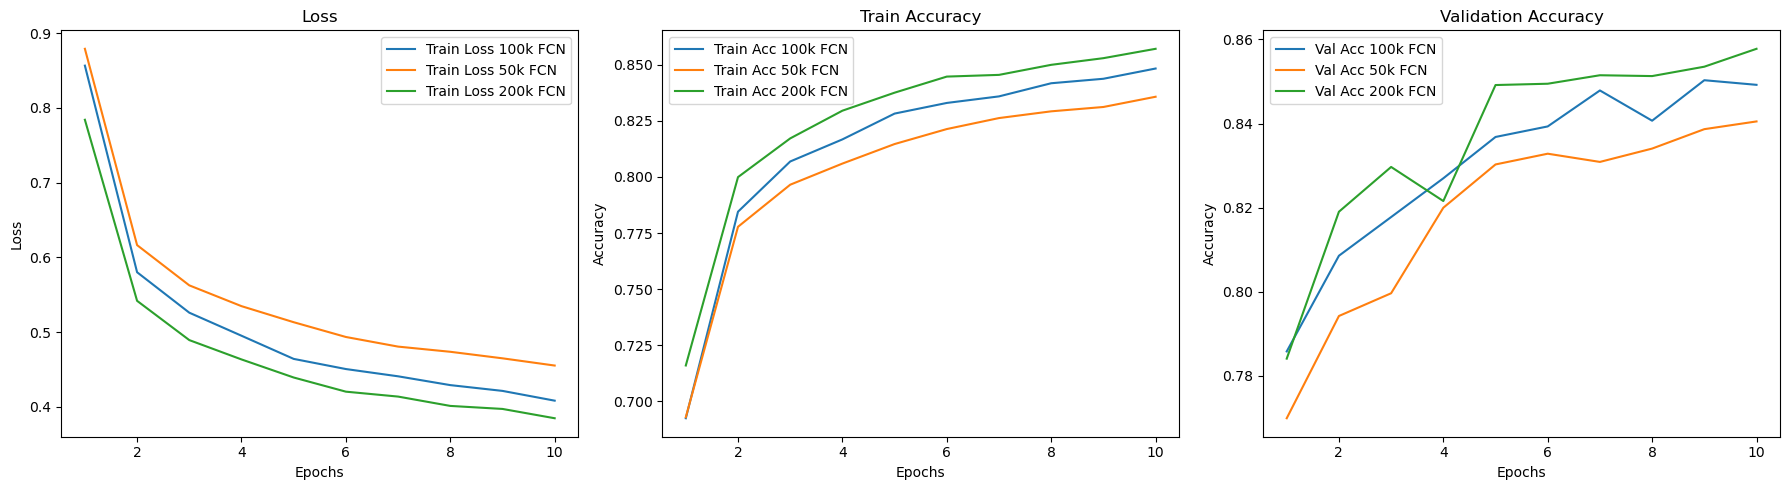
\includegraphics[width=\textwidth]{FCN.png}
    \caption{Training loss and accuracy curves for FCN models}
    \label{fig:FCN}
\end{figure}

In the above figure, we have 3 plots of the Loss curve, Training Accuracy, and Validation Accuracy for 50K, 100K, and 200K FCN models. Overall in all three the generael trend seems to be the same, that the 200K model has the lowest loss and highest accuracy, followed by the 100K model, and then the 50K model.

\begin{figure}[H]
    \centering
    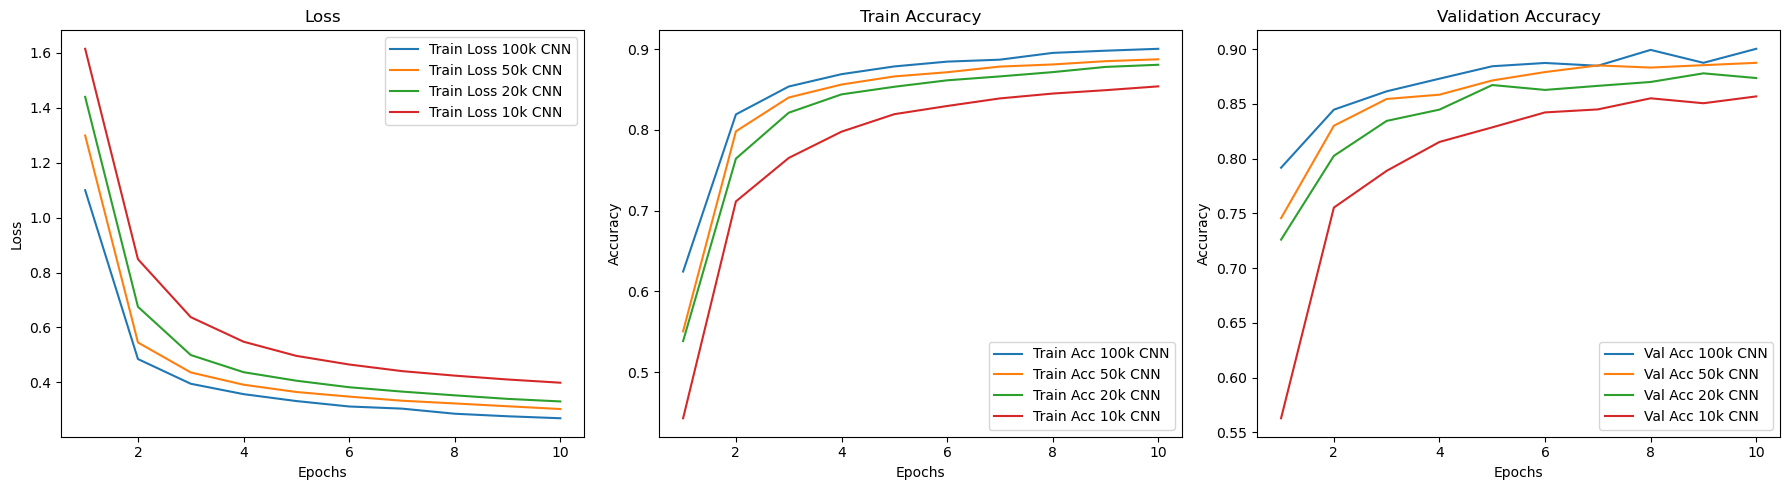
\includegraphics[width=\textwidth]{CNN.png}
    \caption{Training loss and accuracy curves for CNN models}
    \label{fig:CNN}
\end{figure}

Coming into the CNN model, we have 4 plots of the Loss curve, Training Accuracy, and Validation Accuracy for 10K, 20K, 50K, and 100K CNN models. The trend is similar to the FCN model, where the 100K model has the lowest loss and highest accuracy, followed by the 50K model, then the 20K model, and finally the 10K model. However, comparatively, although more data is available in \ref{tab:results}, we can notice the sharper decline in the loss graph, and sharper increase in the accuracy graph for the CNN models.

\begin{table}[H]
\centering
\caption{Summary of Final Training, Validation, and Test Performance}
\begin{tabular}{lcccccc}
\hline
\textbf{Model} & \textbf{Train Loss} & \textbf{Train Acc (\%)} & \textbf{Val Loss} & \textbf{Val Acc (\%)} & \textbf{Test Loss} & \textbf{Test Acc (\%)} \\
\hline
FCN 50K   & 0.4554 & 83.57 & 0.4443 & 84.05 & 0.4077 & 85.73 \\
FCN 100K  & 0.4084 & 84.83 & 0.4059 & 84.92 & 0.3773 & 86.37 \\
FCN 200K  & 0.3849 & 85.71 & 0.3924 & 85.78 & 0.3596 & 87.05 \\
\hline
CNN 10K   & 0.3990 & 85.39 & 0.3939 & 85.69 & 0.4036 & 85.49 \\
CNN 20K   & 0.3308 & 88.06 & 0.3440 & 87.37 & 0.3262 & 88.74 \\
CNN 50K   & 0.3031 & 88.74 & 0.3056 & 88.76 & 0.2953 & 89.29 \\
CNN 100K  & 0.2696 & 90.04 & 0.2577 & 90.04 & 0.2565 & 90.58 \\
\hline
\end{tabular}
\label{tab:results}
\end{table}

\subsection*{Analysis}
Table~\ref{tab:results} presents the key performance metrics across all model variants. A clear trend is observed for the Fully Connected Networks (FCNs): as the parameter budget increases from approximately 50K to 200K, both the training and test accuracies show modest improvements (from 85.73\% to 87.05\% test accuracy). This indicates that while additional parameters allow for learning more complex representations, the improvements are incremental.

On the other hand, the Convolutional Neural Networks (CNNs) demonstrate more significant performance gains. The CNN 100K model achieves the highest test accuracy of 90.58\%, suggesting that the convolutional architecture is particularly well-suited for image data. Even lower-capacity CNN variants, such as the CNN 10K model, perform competitively, although with lower accuracies (85.49\%). In summary, the results indicate that CNN architectures not only converge faster but also generalize better compared to FCNs, especially as the parameter budget increases.

Further analysis of the training curves (loss and accuracy plots) will help illuminate the convergence behavior of each model and provide additional insight into the trade-offs between model complexity and performance.


\section*{Summary and Conclusions}\label{sec:summary}

In this project, we investigated image classification on the Fashion-MNIST dataset using Fully Connected Networks (FCNs) and Convolutional Neural Networks (CNNs) under strict weight budget constraints. Our results demonstrate that while FCNs can achieve competitive performance with limited parameters, CNNs outperform FCNs across all budget levels. The CNN 100K model achieved the highest test accuracy of 90.58\%, highlighting the effectiveness of convolutional architectures for image classification tasks. The training dynamics and performance metrics provide valuable insights into the trade-offs between model complexity, accuracy, and computational efficiency. Future work could explore additional regularization techniques, network architectures, and hyperparameter tuning to further improve performance under weight budget constraints.

\section*{Acknowledgements}\label{sec:acknowledgements}

The author is thankful to Professor Frank for providing the materials and resources needed to complete this assignment. The author is also thankful to the peers Eric Ye and Brighton for discussion on implementing Depthwise Convolution and pseudocode for this project. The author would also like to acknowledge that the code for this project, as well as the Abstract, Introduction and Overview, as well as the theoretical background sections were heavily derived from the Authors own work in Homework 4 of the AMATH 482 course. Lastly, the author would also like to acknowledge that many of the code including building the Neural Network has been discussed in the author's research group since October 2024, as the author is part of the WXML Group on Backdooring ML Models and one of the ML models built was to classify images using a Neural Network, with the dataset being the Fashion-MNIST and MNIST datasets. The research project already involved building CNNs and the author has used inspiration from that project to build the CNNs in this project.


\bibliographystyle{plain}
\bibliography{references}

\end{document}